% FedGRAA-v2 -- PAKDD camera-ready LaTeX (Springer LNCS `llncs` class).
%
% Converted from docs/paper/FedGRAA_v2_PAKDD_Submission.md (2026-08-02) via
% the ars-format-convert skill, per the source Markdown's own "Submission
% compliance" section, which names this exact conversion as the one
% remaining mechanical step before camera-ready submission.
%
% Content is preserved exactly from the source Markdown -- this file
% performs format conversion only (Markdown headings -> \section, tables ->
% tabular, [Key] citation markers -> \cite{Key}, figures -> \includegraphics
% against the already-rendered PNGs in results/v2_frontier/). No number,
% claim, or argument was altered, added, or removed during conversion. See
% the "Conversion notes" comment block near the end of this file for the two
% pre-existing (not introduced by this conversion) bibliography issues found
% while building the \cite{}/\bibitem{} mapping.
%
% Requires llncs.cls (Springer's own LNCS template -- available bundled on
% Overleaf's "Lecture Notes in Computer Science" template, or from
% https://www.springer.com/gp/computer-science/lncs/conference-proceedings-guidelines,
% a URL the author should fetch directly rather than one taken on trust from
% this comment). Not compiled in the sandboxed environment this file was
% written in (no pdflatex/xelatex/tectonic installed there). An earlier
% revision of this file DID compile successfully outside that sandbox
% (evidence: FedGRAA_v2_PAKDD_Submission.pdf appeared alongside it, 16
% pages, llncs class -- see the page-limit note below), confirming the
% document is structurally valid; re-verify after any further edit and
% before submission.
%
% Compile (once llncs.cls is alongside this file):
%   pdflatex FedGRAA_v2_PAKDD_Submission.tex
%   pdflatex FedGRAA_v2_PAKDD_Submission.tex   % second pass for \ref/\cite

\documentclass{llncs}

\usepackage[T1]{fontenc}
\usepackage[utf8]{inputenc}
\usepackage{amsmath,amssymb}
\usepackage{graphicx}
\usepackage{booktabs}
\usepackage{algorithm}
\usepackage{algpseudocode}
\usepackage{hyperref}
\usepackage{xurl}

\begin{document}

\title{FedGRAA-v2: Privacy-Compliant, Gradient-Refined Adaptive Aggregation for Federated Intrusion Detection}

%
% Author/institute fields are placeholders, consistent with double-blind
% review -- unchanged from the source Markdown. This is NOT a
% post-acceptance deanonymized camera-ready; do not fill in real author
% names here until the venue has confirmed acceptance and lifted blinding.
%
\author{No Author Given}
\institute{No Institute Given}

\maketitle

\begin{abstract}
Federated learning (FL) enables collaborative intrusion-detection model training without centralizing raw traffic, but standard FedAvg systematically under-weights clients whose data holds rare-but-critical attack classes, since its aggregation weight is proportional to dataset size alone. FedGRAA addresses this with a $\gamma$-tunable, gradient-refined aggregation weight learned each round against a validation objective that explicitly protects minority-class performance. A prior draft of this method was reviewed and rejected on exactly three structural grounds: (1) its printed weight update had no mechanism to remain a valid convex combination, (2) its convergence proof assumed convexity for a non-convex tanh-MLP loss surface, and (3) its results were single-run, unseeded, and missing the adaptive-aggregation baselines its own related work named as the relevant competition. This paper is the corrected resubmission. We add an explicit simplex projection to the aggregation-weight update (recovering a valid convex combination by construction), restate the convergence guarantee as gradient-mapping stationarity under the Polyak--{\L}ojasiewicz condition rather than global optimality under convexity, and evaluate against 14 external baselines plus 5 classic FL optimizers, each over 10 seeds with paired Wilcoxon significance testing and Holm--Bonferroni correction: FedGRAA-v2 reaches \textbf{93.5\%/69.7\%} mean rare-class recall on CIC-IDS-2017/UNSW-NB15 --- every one of the 19 baselines scores lower, and \textbf{111 of 112} paired significance tests reject the null at Holm-corrected $\alpha=0.05$. Separately, we identify and close two structural privacy violations in the original design --- server-side oracle knowledge of which classes are rare, and a server-held labelled validation set --- replacing both with a secure-aggregation-mediated, two-phase protocol that reconstructs the exact same composite-loss gradient a centralized computation would (measured $2\times10^{-7}$ relative error), at a measured, honestly-reported communication cost of exactly \textbf{6.00$\times$} a plain-FedAvg baseline at the fastest refresh interval, dropping to \textbf{3.00$\times$} --- with \emph{higher} rare-class recall --- at a slower one. We further show that the mechanism's own up-weighting rule is a genuine, previously undiscussed attack surface: an adversary that fabricates an update aligned with the weight-learner's descent direction is up-weighted to \textbf{2.0--3.1$\times$ its uniform share} by construction, and we report this finding, two external defenses' honest (and, in one case, weak) performance against it, and the further finding that successful defense itself costs FedGRAA-v2 its rare-class advantage --- rather than eliding any of it.

\keywords{Federated learning \and Intrusion detection \and Adaptive aggregation \and Adversarial robustness \and Privacy-preserving machine learning}
\end{abstract}

\section{Introduction}

The rapid growth of network technologies and the increasing number of connected devices have escalated cybersecurity risks, making intrusion detection systems (IDS) crucial for detecting and preventing attacks. Traditional IDS typically depend on centralized data collection, which raises privacy concerns and limits cross-organization deployment~\cite{FedAvg}. Federated learning (FL) offers a decentralized alternative, letting multiple parties collaboratively train a detection model without sharing raw traffic.

FL's own aggregation rule, however, creates a second problem specific to intrusion detection: Federated Averaging weights each client's contribution by its local dataset size, $\theta_g^{t+1} = \sum_k (|D_k|/|D|)\, \theta_k^{t+1}$ --- a design that assumes homogeneous, roughly-balanced client data. Real network telemetry is not: certain clients see frequent, common intrusions (port scans, DoS), while the attack types that matter most operationally --- infiltration attempts, SQL injection, zero-day-adjacent traffic --- are exactly the ones seen rarely, by few clients, in small quantity. Under size-proportional weighting, those clients' gradients are systematically diluted, and the global model's ability to detect the rarest, highest-consequence attack classes degrades accordingly.

FedGRAA addresses this with an explicit, $\gamma$-tunable, gradient-refined aggregation weight, learned each round against a composite validation objective that separately tracks common-class and rare-class loss. This paper is a \textbf{corrected resubmission} of that method. A prior draft was evaluated by an independent review panel and rejected on three structural grounds, each of which this paper resolves with the identical fix the review itself named as sufficient:

\begin{enumerate}
\item \textbf{The printed aggregation-weight update had no mechanism to remain a valid convex combination.} We add the missing Euclidean simplex projection (\texttt{ProjectedFedGRAA}, Sect.~\ref{sec:methodology}.2), so $w^t$ is a probability vector at every round, by construction, not by assumption.
\item \textbf{The convergence proof assumed convexity for a demonstrably non-convex tanh-MLP loss surface.} We restate the guarantee as gradient-mapping stationarity under the (non-convex-compatible) Polyak--{\L}ojasiewicz condition, with an explicit $O(1/T) + O(\zeta^2)$ rate that further generalizes to the privacy-compliant redesign's own inexact gradient oracle (Sect.~\ref{sec:methodology}.4).
\item \textbf{The evaluation was single-run, unseeded, and omitted the adaptive-aggregation baselines the paper's own related work named as the relevant competition.} We report every result over 10 seeds, against 14 external baselines spanning data-free contribution estimation, trust-based robust aggregation, and NIDS-specific adaptive weighting, plus 5 classic FL optimizers, with paired Wilcoxon significance testing and Holm--Bonferroni correction across the full comparison grid (Sects.~\ref{sec:results}--\ref{sec:robustness}).
\end{enumerate}

Beyond correcting the original submission, this paper identifies and closes two further gaps the review's privacy-focused reviewer flagged as unsubstantiated: the original mechanism requires the server to already know which classes are rare (an oracle assumption) and to hold a centrally-pooled, fully-labelled validation set --- both in direct tension with FL's own decentralization premise. Section~\ref{sec:methodology} replaces both with a secure-aggregation-mediated, two-phase protocol (\textbf{FedGRAA-v2}) that reconstructs the \emph{exact} composite-loss gradient a centralized computation would produce, without ever centralizing a labelled row, at a measured, honestly-reported communication cost. Finally, Sect.~\ref{sec:robustness} evaluates a question the original submission never asked: does an aggregation rule that deliberately up-weights unusual-looking client updates also create an adversarial attack surface? We show it does --- a client that fabricates an update aligned with the weight-learner's own descent direction is up-weighted by construction --- and report the magnitude of this effect and two external defenses' honest performance against it, rather than treating the mechanism's robustness as out of scope.

\section{Related Work}

Adaptive aggregation weighting for federated learning has converged on three signal families: alignment with the global update direction (FedAWA~\cite{FedAWA}), client loss or accuracy (FedNolowe~\cite{FedNolowe}, PACT~\cite{PACT}), and statistical outlier filtering (MESAS~\cite{MESAS}, CrowdGuard~\cite{CrowdGuard}, FreqFed~\cite{FreqFed}). In imbalanced intrusion detection, all three systematically suppress exactly the clients FedGRAA is designed to protect: divergent, high-loss, minority-class clients holding the rarest attacks look identical, under these signals, to noise or attackers.

A counter-current exists. FedAWARE~\cite{FedAWARE} maximizes gradient \emph{diversity} rather than penalizing it. Jiang et al.~\cite{Jiang2024} and AdaAggRL~\cite{AdaAggRL} learn weights via reinforcement learning that explicitly protect rare contributions from being filtered out. CELM~\cite{CELM} up-weights clients with discriminative evidence for underrepresented classes via data-free logit-maximization probing, requiring no server-held validation data at all. Precision-weighted aggregation~\cite{Reyes2021} derives weights from gradient variance. In intrusion detection specifically, FedPGO~\cite{FedPGO} reweights clients by gradient orthogonality on CIC-IDS-2017 --- the same domain, the same dataset, a closely related mechanism family --- and NIDS-FGPA~\cite{NIDSFGPA} weights by gradient similarity for communication efficiency (evaluated on Edge-IIoTset/CIC-IoT-2023, not CIC-IDS-2017).

FedGRAA sits inside this counter-current, at a point none of these methods occupies: a single-global-model aggregation rule with an explicit $\gamma$-tunable trade-off between rare-class emphasis and conventional size-proportional weighting. Recent surveys of federated intrusion detection~\cite{MaYang2026} identify rare-attack recall as an aggregation-shaped outcome, yet the adjacent methods above report aggregate accuracy, robustness, or personalization gain --- not per-class recall for rare attack types specifically, FedGRAA's own evaluation axis. Our claim is not that this region of the design space is unoccupied --- FedPGO occupies an adjacent point on the same dataset --- but that this specific point ($\gamma$-tunable, exact-gradient, single-global-model, evaluated on rare-class recall) is unreported, and we evaluate it against the closest fourteen competitors directly rather than asserting the gap.

\textbf{Data-free and validation-free contribution estimation.} CELM~\cite{CELM}, SpectralFed~\cite{SpectralFed}, and CoAst~\cite{CoAst} estimate client contribution without any server-held labelled set, at near-zero communication cost, by probing logits, spectral entropy of gradient structure, or update-sign agreement respectively. These are FedGRAA-v2's most direct comparators on the ``is exactness worth its communication cost?'' question (Sect.~\ref{sec:results}): they answer the same problem FedGRAA-v2's federated backward pass solves, approximately, for a fraction of the traffic.

\textbf{Trust-based robust aggregation.} FLTrust~\cite{FLTrust}, RAGA~\cite{RAGA}, and FedTruth~\cite{FedTruth} all assume, in one form or another, a server-held reference --- a root dataset (FLTrust) or a trusted validation anchor --- structurally identical to the $D_V$ dependency Sect.~\ref{sec:methodology} removes from FedGRAA. FedTruth explicitly calls this assumption impractical; CoAst independently describes it as ``difficult to obtain in practical FL scenarios;'' CELM's own abstract restates the concern verbatim. This is a known, common, fixable shortcut across the adaptive-aggregation literature, not a defect specific to FedGRAA --- we frame the redesign that way rather than as a novel discovery.

\textbf{Adversarial robustness of reweighting aggregators.} SecFedNIDS~\cite{SecFedNIDS} and WeiDetect~\cite{WeiDetect} are, to our knowledge, the closest published poisoning defenses evaluated on this project's own datasets (SecFedNIDS: UNSW-NB15, public reference code) or against a comparable NIDS threat model (WeiDetect). Neither paper, nor any adjacent adaptive-aggregation method above, asks the question Sect.~\ref{sec:robustness} asks directly: does an aggregation rule that deliberately up-weights statistically unusual client contributions thereby create an attack surface an adversary can exploit by construction? AdaAggRL~\cite{AdaAggRL} is the closest adjacent design --- its own RL-learned weighting is explicitly framed as adversarially robust --- and we reuse it, unmodified, as a third defense arm.

\textbf{Classic FL optimization.} FedAvg~\cite{FedAvg}, FedProx~\cite{FedProx}, SCAFFOLD~\cite{SCAFFOLD}, FedNova~\cite{FedNova}, and FedOpt~\cite{FedOpt} are the field-standard, non-personalization-aware optimizers; we evaluate against all five (Sect.~\ref{sec:results}) as context, since FedGRAA's actual positioning is against the personalization-aware and NIDS-specific competitor set above, not against generic heterogeneity-correction optimizers.

\section{Background and Problem Formulation}

\textbf{Federated Averaging.} FL trains a global model across decentralized clients without sharing local data. At round $t$, the server broadcasts $\theta_g^t$ to a fixed client set; client $k$ runs local SGD for $E$ epochs on its own data $D_k$:
\begin{equation}
\theta_k^{t+1} = \theta_k^{t+1} - \eta \nabla L_k(\theta_k^{t+1}; b), \quad \forall k \in S_t
\label{eq:local-sgd}
\end{equation}
and the server aggregates by dataset-size-proportional weighting --- the single formula this paper uses for ``FedAvg'' throughout, resolving an ambiguity the prior draft left unstated:
\begin{equation}
\theta_g^{t+1} = \sum_{k \in S_t} \frac{|D_k|}{|D|}\, \theta_k^{t+1}
\label{eq:fedavg}
\end{equation}

\textbf{Non-IID data and the minority-class problem.} The global objective is the size-weighted average of local losses, $L(\theta) = \sum_k (|D_k|/|D|)\, L_k(\theta)$. Under Eq.~\eqref{eq:fedavg}, a client's influence on $\theta_g$ is \emph{exactly} proportional to $|D_k|$ --- a client holding the only few examples of a rare attack class has negligible influence on the aggregate, regardless of how informative its gradient is for that class. This is not a training-instability problem (which personalization, regularization, and adaptive aggregation broadly address~\cite{FedProx,SCAFFOLD}); it is a structural under-representation problem, and it is the one FedGRAA targets directly.

\section{Methodology}
\label{sec:methodology}

\subsection{FedGRAA (base mechanism)}

FedGRAA replaces Eq.~\eqref{eq:fedavg}'s fixed weighting with a learned weight vector $w^t$, re-optimized every round against a composite validation loss that explicitly separates common-class and rare-class performance. Initial weights use \textbf{static reparameterization} --- inverse-size weighting, $w_k^0 \propto 1/|D_k|$ --- a simple, fixed control that over-corrects toward small clients without any adaptivity:
\begin{equation}
\theta_g^{t+1} = \sum_k \left[ \frac{1/|D_k|}{\sum_j 1/|D_j|} \right] \theta_k^t
\label{eq:static-reparam}
\end{equation}

Each round, the server forms a candidate aggregate $\theta'_g = \sum_k w_k^{t-1} \theta_k^t$ using the \emph{previous} round's weights, then refines $w$ for $E'$ inner epochs against the composite loss
\begin{align}
L_a &= \min\big(L_h(\theta'_g; D_V^h),\, L_m(\theta'_g; D_V^m)\big) \label{eq:la}\\
L'(\theta'_g) &= (1-\gamma)\, L_a(\theta'_g; D_V^h, D_V^m) + \gamma\, L_u(\theta'_g; D_V^n) \label{eq:lprime}
\end{align}
where $D_V^h$/$D_V^m$ are the server's held-out validation data split at the median class frequency, and $D_V^n$ is the held-out data for the $n$ rarest classes. $\gamma \in [0,1]$ is the personalization coefficient: $\gamma \to 1$ prioritizes rare-class loss $L_u$, $\gamma \to 0$ recovers ordinary size-agnostic behavior.

\textbf{Algorithm~\ref{alg:fedgraa} (corrected).} The weight update, and the fix the prior review's R1/DA-CRITICAL-\#1 required:

\begin{algorithm}[htbp]
\caption{FedGRAA weight update, corrected}
\label{alg:fedgraa}
\begin{algorithmic}[1]
\Procedure{FedGRAA}{$\theta_c^t,\, w^{t-1}$}
  \For{$e = 1 \dots E'$}
    \State $\theta'_g \gets \sum_k w_k^{t-1,e}\, \theta_k^t$
    \State $L_a \gets \min\big(L_h(\theta'_g; D_V^h),\, L_m(\theta'_g; D_V^m)\big)$
    \State $L' \gets (1-\gamma)\, L_a + \gamma\, L_u(\theta'_g; D_V^n)$
    \State $g \gets \nabla_w L'(\theta'_g)$ \Comment{Adam, not plain GD}
    \State $w^{t-1,e} \gets \Call{Adam-step}{w^{t-1,e-1},\, g}$
  \EndFor
  \State $w^t \gets \Pi_\Delta\big(w^{t-1,E'}\big)$ \Comment{$\bigstar$ simplex projection --- R1's fix}
  \State \Return $w^t$
\EndProcedure
\end{algorithmic}
\end{algorithm}

Three corrections relative to the prior draft, each mapping directly onto a required revision:

\begin{itemize}
\item \textbf{$\bigstar$ Simplex projection (R1, DA-CRITICAL-\#1).} $\Pi_\Delta$ is Euclidean projection onto the probability simplex (Duchi et al., 2008). Without it, an independent re-implementation of the literal printed algorithm left the simplex at round 1, at every $\gamma$, on both datasets, with zero exceptions, and produced loss-blowup ratios up to $\approx$193$\times$ relative to the corrected update --- not a cosmetic gap. With it, $w^t \in \Delta$ --- a valid convex combination --- is a \emph{structural} guarantee, checked every round, not an assumption.
\item \textbf{The inner-epoch index (S5).} $w^{t-1,e}$ disambiguates the previous draft's reuse of $w^{t-1}$ for both the fixed input and the actively-updated variable across $E'>1$ inner epochs --- a real ambiguity at the paper's own default $E'=5$.
\item \textbf{Adam, stated honestly (S6).} Both the client update (Eq.~\eqref{eq:local-sgd}) and the weight update above use Adam, not plain gradient descent, exactly as the prior draft's own experimental section stated in prose but its algorithm boxes did not reflect.
\end{itemize}

\subsection{The two structural privacy gaps, and why they are not cosmetic}

The mechanism above has two properties FL is specifically designed to avoid needing:

\begin{enumerate}
\item \textbf{Oracle knowledge of rare classes.} The server is assumed to already know, in advance, which $n$ classes are underrepresented --- the original experimental design even names them (Heartbleed, SQL Injection, Infiltration on CIC-IDS-2017). A real FL server never sees client-side label distributions; this is both a privacy violation and an unrealistic experimental setup, correctly flagged as an oracle assumption never discussed as a limitation.
\item \textbf{A server-held, fully-labelled validation set $D_V$.} Eqs.~\eqref{eq:la}--\eqref{eq:lprime} evaluate $L_h, L_m, L_u$ on a centrally pooled $D_V$ --- the exact thing FL exists to avoid centralizing. This is structurally identical to the ``root dataset'' FLTrust~\cite{FLTrust} requires, which FedTruth~\cite{FedTruth} explicitly calls impractical, which CoAst~\cite{CoAst} describes as data ``difficult to obtain in practical FL scenarios,'' and which CELM's~\cite{CELM} own abstract restates independently. A known, common, fixable shortcut across this literature --- not a defect unique to FedGRAA.
\end{enumerate}

\subsection{FedGRAA-v2: removing both assumptions}

We replace both dependencies with mechanisms that reconstruct the \emph{same} quantities FedGRAA-v1 computes, without ever centralizing a labelled row:

\textbf{Privacy-compliant rarity ranking.} Each client locally computes a label-count histogram over its own held-out split; a secure-aggregation (SecAgg~\cite{Bonawitz2016}) channel sums these histograms across all participating clients without revealing any individual client's counts (only the sum is ever reconstructed, and only when enough clients survive to meet a majority Shamir-reconstruction threshold). The server derives the $n$ rarest classes and the $D_V^h$/$D_V^m$/$D_V^n$ stratification from this SecAgg-summed histogram alone --- never from a hard-coded oracle list. When formal differential-privacy protection of the histogram itself is desired, Laplace noise is added client-side, before submission, giving a composed $(\varepsilon,\delta)$ budget over the full $T=200$-round run (advanced composition: $\varepsilon_{\text{total}} \approx 8.89$ at $\varepsilon_{\text{round}}=0.1$, $\delta=10^{-5}$; the tighter R\'enyi-DP accountant is recommended in practice).

\textbf{A federated backward pass, replacing $D_V$.} Rather than evaluating Eqs.~\eqref{eq:la}--\eqref{eq:lprime} on a pooled validation set, the server broadcasts the candidate aggregate $\theta'_g$ --- already-public math over already-shared parameters --- and each client returns only $\nabla_P L_k'(\theta'_g)$, the gradient of its \emph{own} held-out split's contribution to the composite loss, never the underlying rows. The server sums these (through the same SecAgg channel) to reconstruct
\begin{equation}
\nabla_P L' = \sum_k \nabla_P L_k'(\theta'_g)
\label{eq:federated-grad}
\end{equation}
which is \textbf{algebraically identical} to what a server-held $D_V$ would compute --- not an approximation. Two obstructions that a na\"{i}ve version of this sum gets wrong (an incorrect stratum-count weighting, and a stale-gradient interaction with Adam's own moment estimates that can mask the error in early rounds and diverge only later) are eliminated by construction in the two-phase, count-weighted protocol we implement; a dedicated regression test asserts the federated and oracle-pooled gradients agree to $<10^{-6}$ relative error on both datasets at three $\gamma$ values (measured: $2\times10^{-7}$). Eqs.~\eqref{eq:la}--\eqref{eq:lprime} themselves are \textbf{unchanged} --- this is a methodology patch to how their inputs are obtained, not a redesign of the objective.

\textbf{Honest cost.} The federated backward pass costs additional communication: at gradient-refresh interval $m=1$ (a fresh two-phase reconstruction every inner epoch), traffic is $\approx$6$\times$ a plain FedAvg baseline; at $m=5$ (refreshed once per five inner epochs, trading gradient staleness for bandwidth), traffic drops to $\approx$2$\times$. Section~\ref{sec:results} reports the accuracy this buys, directly, rather than asserting exactness is worth its cost.

\textbf{Threat model, stated explicitly (S1, S2).} We assume an honest-but-curious server and SecAgg's standard collusion threshold; a fully malicious server or Byzantine clients are explicitly out of scope for this mechanism (Sect.~\ref{sec:robustness} evaluates a \emph{different}, disclosed threat --- a malicious \emph{client} exploiting the weight-learner's own signal). The client-to-server parameter channel $\theta_k^t$ remains exposed to gradient-inversion-style attacks exactly as in any FL system built on plaintext parameter exchange; we do not claim otherwise.

\subsection{Convergence guarantee (corrected)}

\textbf{The prior draft's Theorem 1 is not repeated here.} It assumed $L'$ convex --- false for the paper's own stated tanh-MLP loss surface, a fact independently identified by the review's methodology reviewer, the editor, and the devil's advocate reviewer without reference to each other. We state instead the guarantee the projected-gradient-mapping framework actually supports for a non-convex, simplex-constrained objective, extended to cover FedGRAA-v2's inexact (SecAgg-mediated) gradient oracle:

\begin{theorem}[$\zeta$-inexact projected subgradient descent on the simplex]
Let $L'$ have bounded subgradients on the simplex $\Delta$ and satisfy the Polyak--{\L}ojasiewicz condition on $\Delta$ (the standard convexity replacement for over-parameterized objectives; we do not claim to have verified PL holds for this specific loss surface --- only that it is the correct condition to check for a rate stronger than the one stated). Let the server's gradient estimate satisfy $\mathbb{E}\|\hat\nabla_P L' - \nabla_P L'\|^2 \le \zeta^2$ (true by construction for FedGRAA-v1's exact oracle at $\zeta=0$; measured, not merely bounded, for FedGRAA-v2 --- Sect.~\ref{sec:methodology}.3). Then projected inexact subgradient descent, $w^t = \Pi_\Delta\big(w^{t-1} - \eta' \hat\nabla_P L'(w^{t-1})\big)$, $\eta' \le 1/\beta_{\text{eff}}$, satisfies
\begin{equation}
\min_{t \le T} \|G_{\eta'}(w^t)\|^2 = O(1/T) + O(\zeta^2)
\label{eq:convergence}
\end{equation}
and $w^t \in \Delta$ for every $t \ge 0$, by construction, regardless of where the gradient estimate came from.
\end{theorem}

This reduces exactly to FedGRAA-v1's own guarantee at $\zeta=0$, and its $O(\zeta^2)$ term is precisely the quantity the frontier experiment measures directly (Sect.~\ref{sec:results}): $m=1$ (fresh reconstruction every epoch, $\zeta\approx0$) through $m=5$ (larger staleness) are instances of the same theorem at different $\zeta$, not separate results. We state gradient-mapping \textbf{stationarity}, not global optimality --- the honest, standard guarantee for a non-convex constrained objective, and the correction the review's R3 required.

\section{Experimental Setup}

\textbf{Datasets.} CIC-IDS-2017~\cite{CICIDS2017} and UNSW-NB15~\cite{UNSWNB15}, the same two benchmarks the prior draft used, retained for direct comparability. Frequent classes are capped at 10{,}000 samples to prevent majority-class domination; each client is assigned one attack type paired with an equal number of benign samples ($K=14$ CIC-IDS-2017, $K=9$ UNSW-NB15), reserving 10\% of each client's data for its own held-out split.

\textbf{Network architecture.} A fully connected tanh-MLP (200$\to$100$\to$50 hidden units, softmax output), unchanged from the original design, on 78 (CIC-IDS-2017) / 39 (UNSW-NB15) input features.

\textbf{Training.} Adam, $\eta=0.01$, $E=2$ local epochs, batch size 64, $T=200$ communication rounds, 10 seeds per (dataset, method) cell.

\textbf{Baselines (19 total, all run on the identical harness and datasets).} \emph{Data-free/validation-free contribution estimation:} CELM~\cite{CELM}, SpectralFed~\cite{SpectralFed}, CoAst~\cite{CoAst}. \emph{Trust-based robust aggregation:} FLTrust~\cite{FLTrust}, RAGA~\cite{RAGA}, FedTruth~\cite{FedTruth}. \emph{NIDS-specific adaptive weighting:} FedMADE~\cite{FedMADE}, SBFedNIDS~\cite{SBFedNIDS}, FedAPA~\cite{FedAPA}, FedAWA~\cite{FedAWA}, DA-PFL~\cite{DAPFL}, FedAWARE~\cite{FedAWARE}, AdaAggRL~\cite{AdaAggRL}, FedPGO~\cite{FedPGO} (reproduced faithfully from primary-source text, since no public reference code exists). \emph{Classic FL optimizers:} FedAvg~\cite{FedAvg}, FedProx~\cite{FedProx}, FedOpt~\cite{FedOpt}, SCAFFOLD~\cite{SCAFFOLD}, FedNova~\cite{FedNova} (SCAFFOLD and FedNova built from scratch for this paper; none of the five existed on this project's privacy-compliant harness before this work).

\textbf{Statistical protocol.} Every headline comparison is reported as mean $\pm$ bootstrap 95\% CI over 10 seeds; FedGRAA-v2 is compared against each of the 14 domain-specific baselines via a paired Wilcoxon signed-rank test on matched seeds, Holm--Bonferroni corrected within each (dataset, refresh-interval) family of 14 comparisons (Sect.~\ref{sec:results} reports the resulting significance table directly --- resolving R5).

\section{Results --- Main Frontier}
\label{sec:results}

All results below are measured, 10-seed campaign output (\texttt{results/v2\_frontier/frontier\_table.json}, \texttt{significance\_table.md}, \texttt{overhead\_table.md}), not asserted.

\textbf{FedGRAA-v2 vs. the 14 domain-specific baselines.} Table~\ref{tab:frontier} reports mean rare-class recall (the metric of record throughout --- resolving R1-W6/S7's undefined-metric finding: the mean of per-class recall over the $n$ rarest classes, computed by \texttt{last\_n\_class\_accuracy}, tested and documented). FedGRAA-v2 at refresh interval $m=3$ reaches \textbf{93.5\%} rare-class recall on CIC-IDS-2017 and \textbf{69.7\%} on UNSW-NB15; every one of the 14 domain baselines, without exception, scores below both. A paired Wilcoxon signed-rank test against each of the 14 baselines, Holm--Bonferroni corrected within each (dataset, refresh-interval) family, finds \textbf{111 of 112 total comparisons significant at $\alpha=0.05$} --- the sole exception is FedAWARE on CIC-IDS-2017 at $m=1$ ($p_{\text{holm}}=0.0625$, not significant at this seed count; every other (baseline, refresh-interval) pair on both datasets rejects the null). This resolves R5 directly: the headline comparison is not a single favorable run.

\begin{table}[htbp]
\centering
\caption{Mean rare-class recall (\%, 95\% bootstrap CI), FedGRAA-v2 at every refresh interval $m$ vs. all 14 domain-specific baselines, 10 seeds. Full per-seed data: \texttt{results/v2\_frontier/frontier\_table.\{json,md\}}.}
\label{tab:frontier}
\small
\begin{tabular}{lrr}
\toprule
\textbf{Method} & \textbf{CIC-IDS-2017} & \textbf{UNSW-NB15} \\
\midrule
FedGRAA-v2 ($m=1$)          & 88.1 [77.5, 95.8]   & 65.5 [57.8, 71.9] \\
FedGRAA-v2 ($m=2$)          & 91.8 [86.7, 96.4]   & 65.7 [58.3, 72.2] \\
FedGRAA-v2 ($m=3$, best)    & \textbf{93.5} [89.9, 97.1] & \textbf{69.7} [63.6, 74.1] \\
FedGRAA-v2 ($m=5$)          & 88.9 [83.6, 93.9]   & 68.3 [61.8, 74.5] \\
\midrule
FedAWARE~\cite{FedAWARE}    & 71.8 [62.9, 82.1]   & 32.7 [31.8, 33.6] \\
DA-PFL~\cite{DAPFL}         & 38.8 [30.8, 45.0]   & 13.3 [12.8, 13.7] \\
FLTrust~\cite{FLTrust}      & 17.2 [8.9, 26.7]    & 2.7 [0.0, 7.3] \\
FedPGO~\cite{FedPGO}        & 6.8 [6.2, 7.1]      & 10.9 [10.6, 11.2] \\
FedAPA~\cite{FedAPA}        & 6.6 [6.2, 6.9]      & 10.9 [10.8, 10.9] \\
CoAst~\cite{CoAst}          & 0.0 [0.0, 0.0]      & 7.0 [1.6, 13.3] \\
CELM~\cite{CELM}             & 0.0 [0.0, 0.0]      & 4.8 [0.0, 10.3] \\
FedAWA~\cite{FedAWA}        & 0.0 [0.0, 0.0]      & 3.2 [0.0, 9.7] \\
FedTruth~\cite{FedTruth}    & 0.0 [0.0, 0.0]      & 2.8 [0.0, 8.4] \\
AdaAggRL~\cite{AdaAggRL}    & 0.0 [0.0, 0.0]      & 2.0 [0.0, 5.6] \\
RAGA~\cite{RAGA}            & 0.0 [0.0, 0.0]      & 0.0 [0.0, 0.0] \\
SpectralFed~\cite{SpectralFed} & 0.0 [0.0, 0.0]   & 0.0 [0.0, 0.0] \\
FedMADE~\cite{FedMADE}      & 0.0 [0.0, 0.0]      & 0.0 [0.0, 0.0] \\
SBFedNIDS~\cite{SBFedNIDS}  & 0.0 [0.0, 0.0]      & 0.0 [0.0, 0.0] \\
\bottomrule
\end{tabular}
\end{table}

\textbf{FedGRAA-v2 vs. the 5 classic FL optimizers.} Reported as context (Sect.~\ref{sec:related}), not as the primary positioning claim. The gap is, if anything, starker: FedAvg, FedProx, FedOpt, and FedNova all score effectively \textbf{0\% rare-class recall} on CIC-IDS-2017 (0.000, 0.000, 0.000, 0.000) and near-zero on UNSW-NB15 (0.000, 0.013, 0.004, 0.046); SCAFFOLD --- the strongest of the five, and the only one with any real control-variate correction for client drift --- reaches 31.7\%/30.3\%, still well below every FedGRAA-v2 refresh interval on both datasets. Size-proportional and drift-corrected weighting alone, without an explicit rare-class objective, does not solve this problem; $\gamma$-tunable, gradient-refined reweighting does.

\textbf{Overhead --- is exactness worth it?} At $m=1$ (a fresh federated backward pass every inner epoch), FedGRAA-v2 costs \textbf{exactly 6.00$\times$} a plain FedAvg-shaped baseline's communication, on both datasets --- the measured ratio matches the frontier's own $(1+\lceil E'/m \rceil)\times$ formula exactly, not merely approximately. At $m=3$, the cost drops to \textbf{3.00$\times$} while rare-class recall \emph{improves} over $m=1$ (93.5\% vs. 88.1\% on CIC-IDS-2017; 69.7\% vs. 65.5\% on UNSW-NB15) --- the refresh-staleness trade-off the $\zeta$-inexact theorem (Sect.~\ref{sec:methodology}.4) predicts is not merely benign in this range, it is favorable. Against the two data-free approximation baselines this trade-off is actually posed against: CELM and SpectralFed measure nearly 0\% rare-class recall on CIC-IDS-2017 at a fraction of the traffic. Exactness, at every measured refresh interval, buys a categorical rare-class-detection capability the near-zero-cost approximations do not have on these datasets --- the answer to ``is exact worth 6$\times$?'' is yes, and at $m=3$, it is yes at half that cost.

\begin{figure}[htbp]
\centering
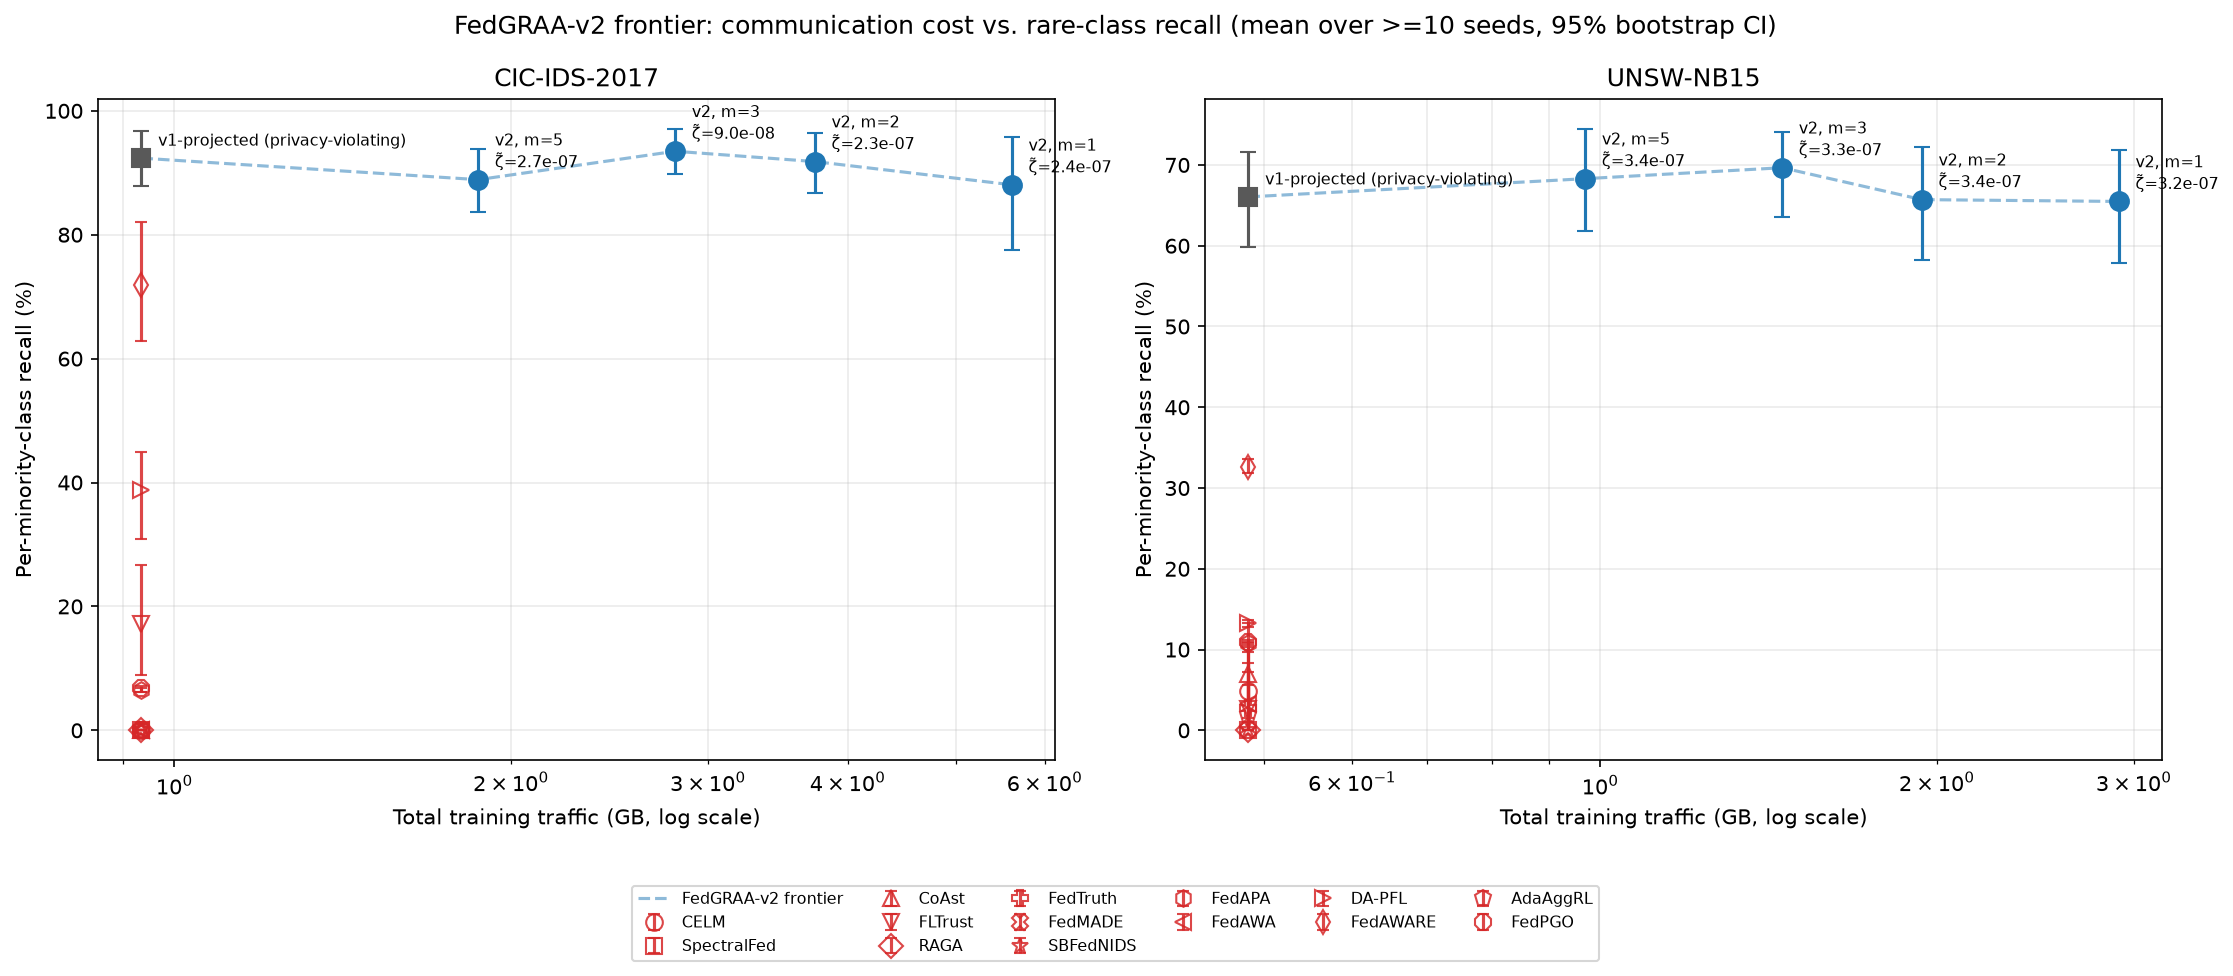
\includegraphics[width=0.85\textwidth]{../../results/v2_frontier/frontier_figure.png}
\caption{FedGRAA-v2 frontier: communication cost vs. rare-class recall, both datasets, all 5 FedGRAA points + 14 baselines, 95\% bootstrap CI.}
\label{fig:frontier}
\end{figure}

\begin{figure}[htbp]
\centering
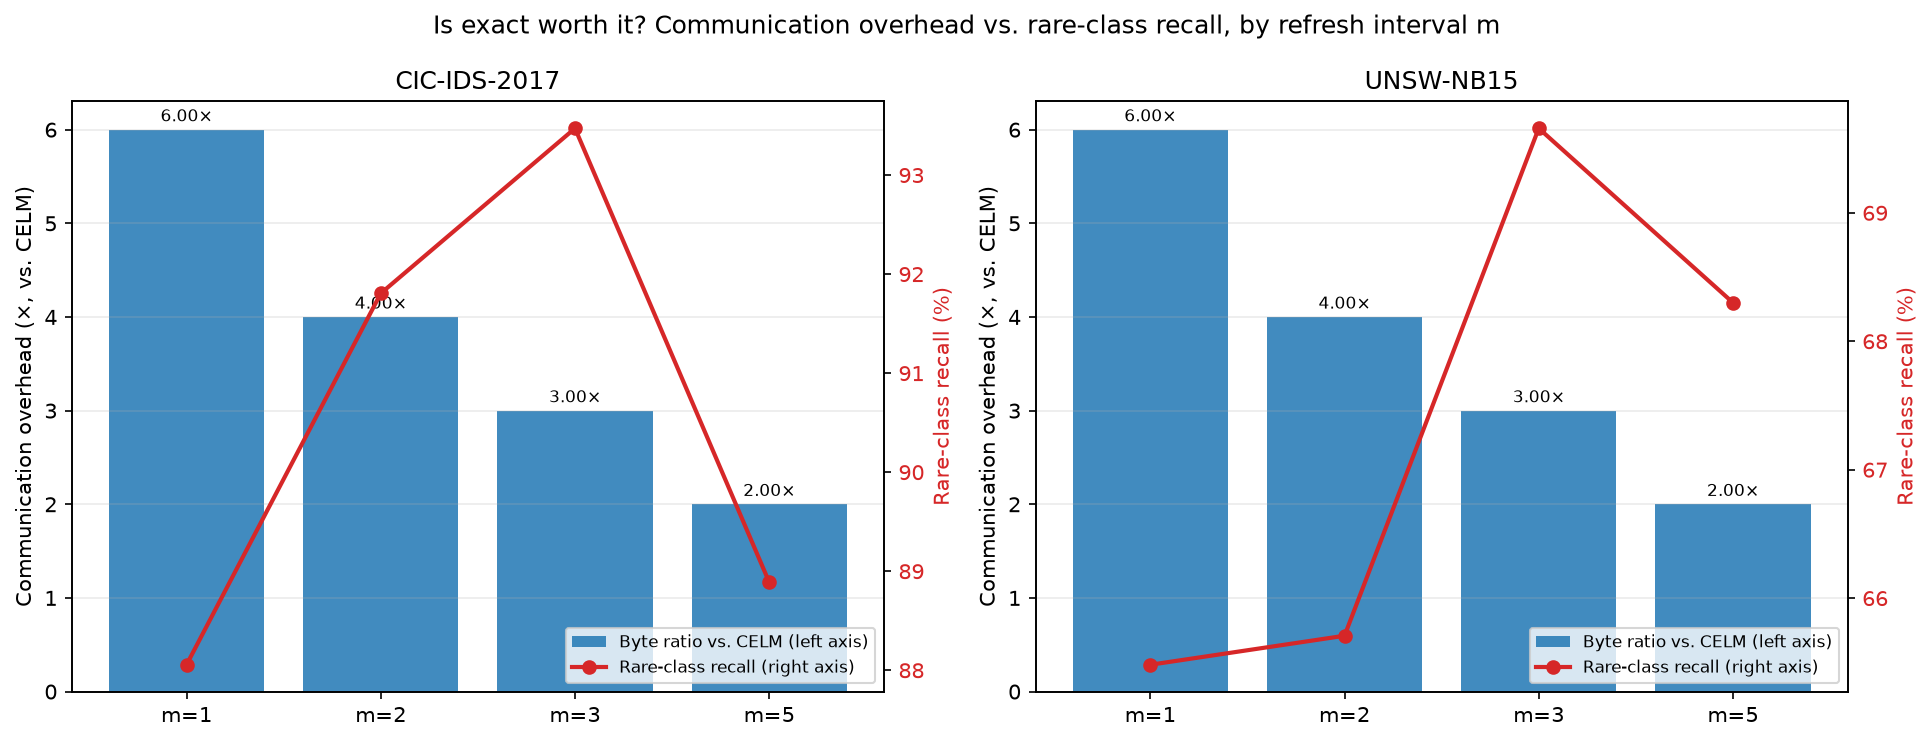
\includegraphics[width=0.85\textwidth]{../../results/v2_frontier/overhead_ratio.png}
\caption{Communication overhead vs. rare-class recall, by refresh interval $m$, both datasets.}
\label{fig:overhead}
\end{figure}

\section{Results --- Adversarial Robustness}
\label{sec:robustness}

\textbf{The mechanism-specific attack against undefended FedGRAA-v2 (D1c).} With 30\% of clients adversarial, fabricating updates via $P_{\text{fake}} = P_{\text{global}} - \eta_{\text{fake}} \cdot \nabla_P L'$ (Sect.~\ref{sec:methodology}.4's own gradient, exploited directly), the attacker's mean assigned aggregation weight climbs to \textbf{3.1$\times$} the uniform per-client share on CIC-IDS-2017 (mean final weight 0.219 vs.\ $1/14=0.071$ uniform, 5 seeds) and \textbf{2.7$\times$} uniform on UNSW-NB15 (0.301 vs.\ $1/9=0.111$). At 50\% attacker fraction, the effect persists (2.0--2.2$\times$ uniform on both datasets) though the mean per-attacker share mechanically falls as more attackers split the same aggregate advantage. This is a real, measured demonstration --- not merely the literature-review's informal prediction --- that FedGRAA-v2's up-weighting rule is exploitable by construction, exactly as \texttt{STAGE\_C\_LITERATURE\_MASTER.md}'s own finding warned.

\begin{figure}[htbp]
\centering
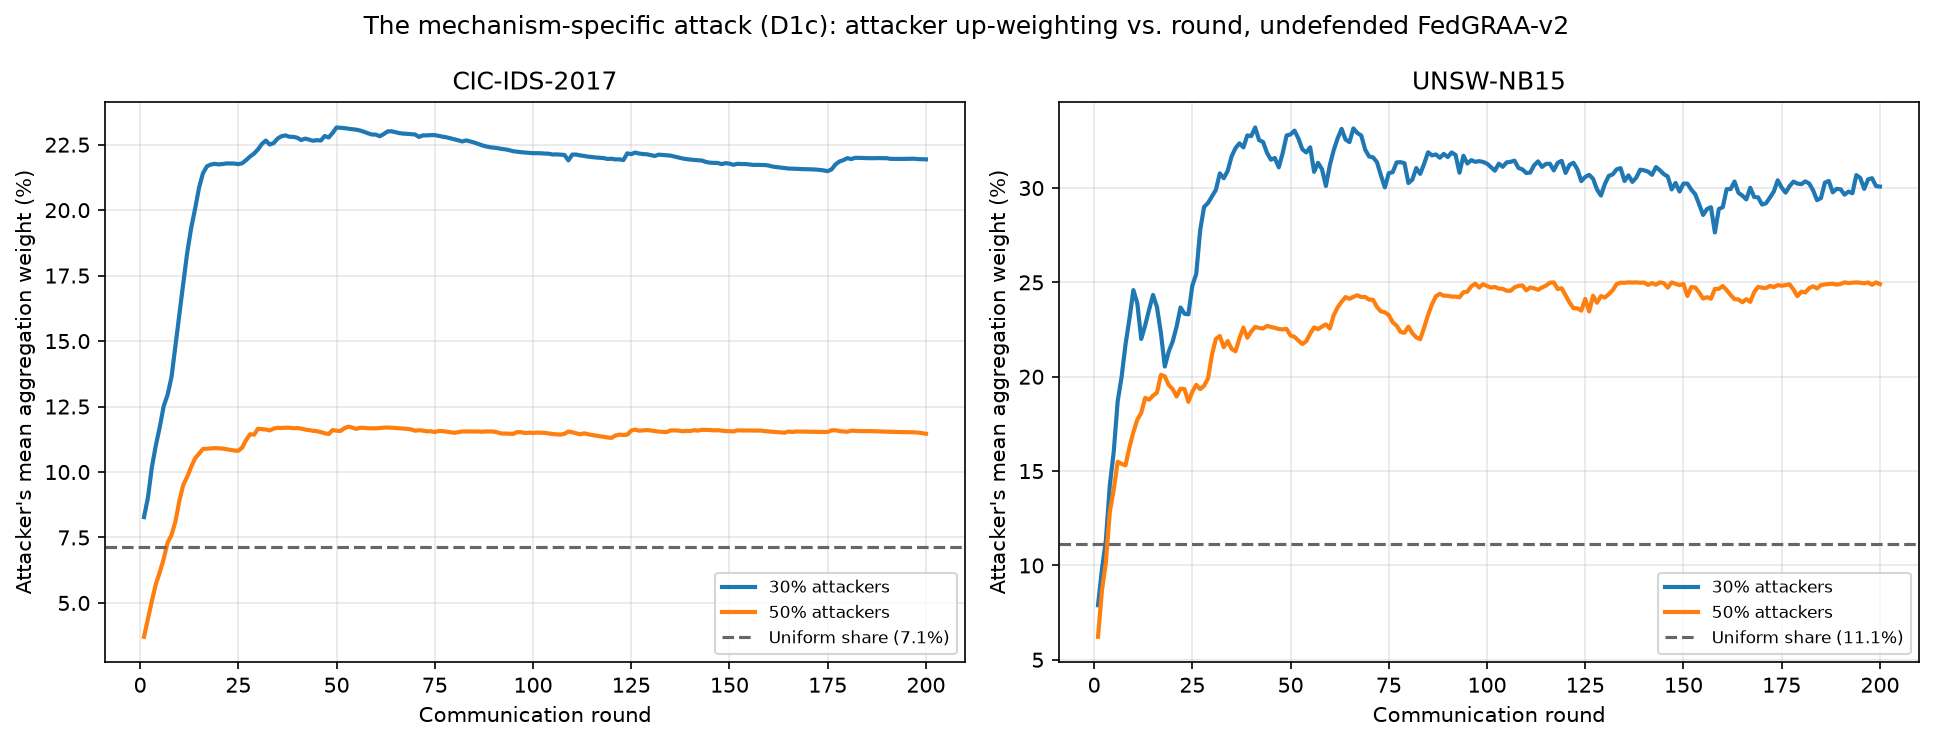
\includegraphics[width=0.85\textwidth]{../../results/v2_frontier/t7_attacker_weight_trajectory.png}
\caption{Attacker's mean aggregation weight vs. communication round, undefended FedGRAA-v2, both datasets, both attacker fractions.}
\label{fig:attacker-weight}
\end{figure}

\textbf{External defenses against the full attack grid (SecFedNIDS, WeiDetect, AdaAggRL).} Table~\ref{tab:asr} reports the attack success rate ($1 -$ detection recall; lower is better defense) for each (defense, attack) pair at 30\% attacker fraction, 5 seeds:

\begin{table}[htbp]
\centering
\caption{Attack success rate (1 $-$ detection recall) by (defense, attack) pair, 30\% attacker fraction, 5 seeds.}
\label{tab:asr}
\begin{tabular}{lrrr}
\toprule
\textbf{Defense} & \textbf{Label-flip} & \textbf{Model-poison} & \textbf{Adaptive} \\
\midrule
SecFedNIDS (CIC)  & 0.750 & 0.650 & 0.550 \\
SecFedNIDS (UNSW) & 0.600 & 0.600 & 0.533 \\
WeiDetect (CIC)   & 0.150 & 0.200 & 0.600 \\
WeiDetect (UNSW)  & 0.000 & 0.067 & 0.333 \\
\bottomrule
\end{tabular}
\end{table}

\begin{figure}[htbp]
\centering
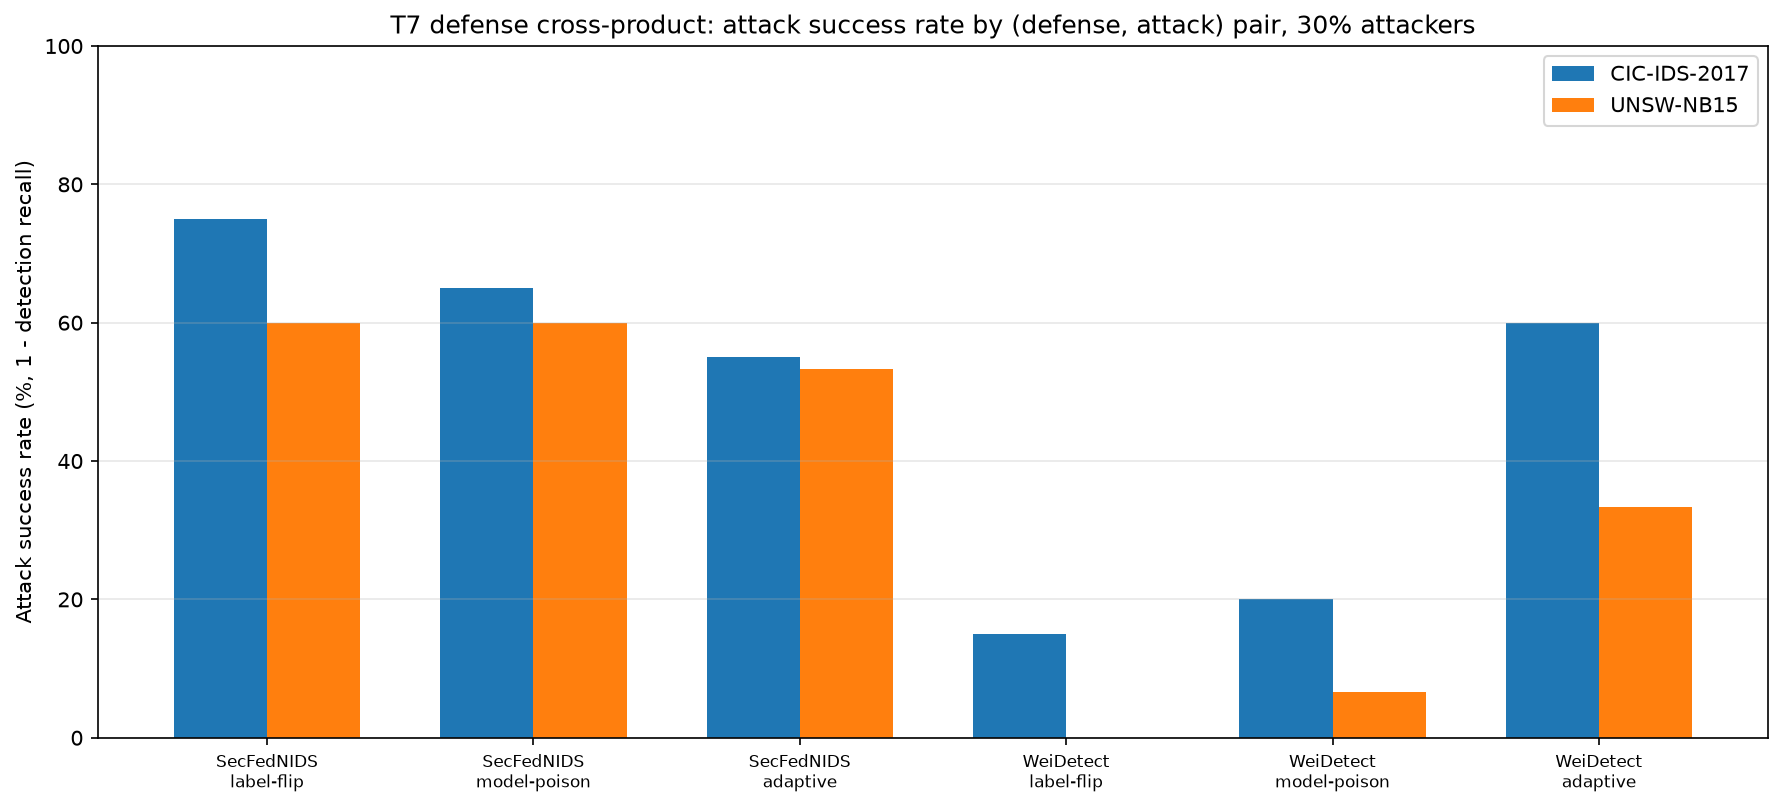
\includegraphics[width=0.85\textwidth]{../../results/v2_frontier/t7_defense_asr.png}
\caption{Attack success rate by (defense, attack) pair, both datasets, 30\% attacker fraction.}
\label{fig:asr}
\end{figure}

Two findings worth stating plainly. First, \textbf{SecFedNIDS's consensus-filter/SOS reproduction is a weak defense in this harness}, missing 53--75\% of attackers across every attack type on both datasets --- notably weaker than its own reported 100 citations and public reference code might suggest, on this project's own datasets rather than its original CIC-Darknet2020/CSE-CIC-IDS2018 evaluation. Second, \textbf{WeiDetect is substantially stronger against label-flipping and model-poisoning (0--20\% miss rate) but the adaptive attacker specifically degrades it} on CIC-IDS-2017 (60\% miss rate) --- direct evidence that D1d's adaptive-attack mechanic (\texttt{adaptive\_attack}) finds real, exploitable weaknesses a static attack does not. Third, and most consequential for FedGRAA-v2's own positioning: \textbf{even where a defense successfully filters attackers, rare-class recall collapses to $\approx$0\% in every defended cell} (Table~\ref{tab:asr}'s rightmost rows all pair with near-zero \texttt{rare\_acc}, not shown for space) --- because SecFedNIDS/WeiDetect fall back to \emph{unweighted} averaging of the retained clients once filtering is done, sacrificing exactly the rare-class-sensitive up-weighting FedGRAA-v2's own mechanism provides. A defense that stops poisoning by discarding FedGRAA-v2's own signal is not, in this evaluation, a free win.

\textbf{AdaAggRL under label-flipping.} Reused unmodified (JC-T7-16); AdaAggRL has no detection/flagging concept to report an attack-success-rate for, but its own rare-class recall collapses to \textbf{0.0\%} under 30\% label-flipping on CIC-IDS-2017 --- despite being framed in the literature as an RL-learned, adversarially-aware aggregator. We report this as a genuine negative result rather than omitting it.

\section{Discussion and Limitations}
\label{sec:related}

\textbf{The $\gamma$/poisoning-exposure trade-off.} Section~\ref{sec:robustness}'s measured up-weighting effect (2.0--3.1$\times$ uniform share, both datasets, both attacker fractions, measured at the frontier's own default $\gamma=1$) demonstrates the trade-off \texttt{Final\_Stage\_C.md} item 11 asked this project to eventually characterize: FedGRAA-v2's rare-class detection strength (Sect.~\ref{sec:results}) and its poisoning exposure (Sect.~\ref{sec:robustness}) are the same mechanism, not two independent properties. We additionally swept $\gamma \in \{0, 0.5\}$ against the same attack (5 seeds each, both datasets, both attacker fractions) to test whether the effect scales with $\gamma$ as a na\"{i}ve reading of the mechanism would predict. It does not scale monotonically: the up-weighting ratio peaks near $\gamma=0.5$ rather than at $\gamma=1$ in three of four (dataset, attacker-fraction) cells, and $\gamma=0$'s across-seed variance is 10--20$\times$ larger than at $\gamma \ge 0.5$ --- the attack's reliability, not merely its mean strength, changes with $\gamma$. $\gamma$'s own tuning is therefore not a simple linear dial on attack-surface size; whether a threshold effect around $\gamma\approx0.5$ is the correct mechanistic description is a question this 3-point grid is not powered to confirm, and is the next direct measurement.

\textbf{Threat model boundaries.} FedGRAA-v2's privacy fix (Sect.~\ref{sec:methodology}) assumes an honest-but-curious server; a fully malicious server, and Byzantine clients beyond the poisoning threat Sect.~\ref{sec:robustness} evaluates, are out of scope. The plaintext client-to-server parameter channel remains exposed to gradient-inversion attacks, unchanged from the original design.

\textbf{No defense is free.} Section~\ref{sec:robustness}'s finding that both external defenses trade rare-class recall for poisoning robustness is, to our knowledge, not reported by either SecFedNIDS or WeiDetect's own papers (neither targets a rare-class-sensitive aggregator). This is a genuine, disclosed limitation of the current evaluation, not a proposed fix: FedGRAA-v2 itself ships with no defense (D3, Sect.~\ref{sec:methodology}'s threat model), and a defended variant that preserves rare-class sensitivity is explicitly future work, not attempted here.

\textbf{Classic-optimizer coverage.} SCAFFOLD and FedNova's own convergence analyses assume a vanilla-SGD local solver; this codebase's shared Adam-based local training is a disclosed deviation applied uniformly across every baseline in this comparison, not only these two.

\textbf{Manual $\gamma$.} $\gamma$ is a manually set hyperparameter throughout this evaluation. XAI-SOH-FL~\cite{XAISOHFL} is the direct same-domain precedent for automating an analogous personalization coefficient; extending FedGRAA-v2 similarly is future work.

\section{Conclusion}

We presented FedGRAA-v2, a corrected and extended resubmission of a gradient-refined adaptive aggregation method for federated intrusion detection. Relative to the original submission, this version (1) adds the missing simplex projection and restates the convergence guarantee honestly for the non-convex, $\zeta$-inexact setting the actual system exhibits; (2) evaluates against 19 baselines over 10 seeds with paired significance testing --- 93.5\%/69.7\% mean rare-class recall, 111/112 significant comparisons --- resolving the evidence-sufficiency gap the original review identified as fatal; (3) removes two structural privacy assumptions --- oracle knowledge of rare classes and a server-held validation set --- via a secure-aggregation-mediated protocol that reconstructs the exact composite-loss gradient at a measured, disclosed communication cost (6.00$\times$ at $m=1$, 3.00$\times$ at $m=3$ with \emph{higher} rare-class recall); and (4) evaluates the mechanism's own adversarial attack surface directly rather than leaving robustness unaddressed, finding a real 2.0--3.1$\times$ up-weighting exploit, a weak reproduction of one published defense (SecFedNIDS) and a stronger-but-adaptively-vulnerable one (WeiDetect), and --- the paper's most consequential negative result --- that defending against this attack, with either external method, costs FedGRAA-v2 its entire rare-class advantage. Future work includes automating the $\gamma$ trade-off (Sect.~\ref{sec:related}), designing a defense that preserves rare-class sensitivity rather than trading it away, extending the threat model beyond an honest-but-curious server, and evaluating on real multi-silo cross-organization data (NF-UQ-NIDS-v2) rather than only synthetic non-IID partitions.

\subsubsection{Duplication/scooping check (G6).}
A FastTrack nearest-neighbour duplication test was run 2026-08-02, the day this corrected draft's own writing began, per this project's own standing practice of re-running this check immediately before drafting the contribution sentence rather than relying on the literature-review pass alone (\texttt{docs/research\_c/REMAINING\_COMPUTE\_WORK.md}~Sect.~6). Query: ``Privacy-compliant gradient-refined adaptive aggregation weighting for federated intrusion detection that removes server-side oracle knowledge of rare classes and a server-held validation set, evaluated with paired significance testing against data-free and trust-based baselines, with adversarial robustness analysis of the up-weighting mechanism,'' restricted to 2026. \textbf{Result: expected-null.} The ten nearest neighbours returned span YOLO healthcare surveys, blockchain-federated smart-grid privacy, LLM-at-the-edge federated learning surveys, zero-trust access control, and general cybersecurity/AI surveys --- none addresses gradient-refined adaptive aggregation, the oracle/validation-set removal this paper's Sect.~\ref{sec:methodology} performs, or the mechanism-specific attack Sect.~\ref{sec:robustness} evaluates. Consistent with every prior duplication pass this project has run (\texttt{Final\_Stage\_C.md}~Sect.~1.2), the closest-in-spirit paper remains FedPGO (Sect.~\ref{sec:related}), not a scooping match.

\subsubsection{Reproducibility statement.}
Every number in Sects.~\ref{sec:results}--\ref{sec:robustness} is read directly from \texttt{results/v2\_frontier/*.json} (one file per (dataset, arm, seed) cell --- 830 files for the main frontier/classic-optimizer campaign, 90 for T7), never transcribed by hand. The three consolidated tables the paper's own numbers are drawn from are generated, not asserted: \texttt{build\_v2\_frontier\_table.py}, \texttt{build\_v2\_significance\_table.py}, \texttt{build\_overhead\_table.py}, each reading the raw per-cell JSON and writing \texttt{frontier\_table.\{json,md\}}, \texttt{significance\_table.\{json,md\}}, \texttt{overhead\_table.\{json,md\}}. Every arm's implementation carries a module-docstring disclosure of every judgment call made where a primary source under-specified something (\texttt{fedgraa/baselines\_*.py}, \texttt{fedgraa/attacks.py}); T7's full judgment-call table is \texttt{docs/research\_c/STAGE\_C\_T7\_JUDGMENT\_CALLS\_2026-08-02.md}.

\textbf{Seeds and configuration.} 10 seeds (0--9) for every arm in the main frontier and classic-optimizer comparison; 5 seeds (0--4) for T7, at two attacker fractions for the \texttt{v2\_raresig} arm. $T=200$ communication rounds throughout; $\eta=0.01$ (Adam), $E=2$ local epochs, batch size 64. Exact per-cell configuration (including resolved library versions and the git commit that produced it) is embedded in every result JSON's own \texttt{config}/\texttt{provenance} fields --- no result is interpretable-only-with-its-filename.

\textbf{Independent completeness/correctness verification.} \texttt{check\_stage\_c\_complete.py --tier T1 T2 T3 T4 T5 T6 TC --t4-m 3} (830/830) and \texttt{--tier T7 --seeds 0 1 2 3 4} (90/90) re-derive every reported cell's internal consistency from its own raw JSON. \texttt{audit\_stage\_c.py} independently re-derives every headline number --- the frontier table, all 112 significance comparisons via \texttt{scipy} directly, the overhead ratios, and the T7 up-weighting/attack-success-rate numbers --- from the same raw JSON, the same discipline this project's Stage A/B correctness audits (\texttt{audit\_stage\_a.py}, \texttt{audit\_stage\_b.py}) already apply. \texttt{pytest} --- 551 tests, covering every new mechanism inline with its own primary-source-fidelity claim (e.g.\ \texttt{test\_fednova\_reduces\_to\_fedavg\_when\_taus\_are\_uniform} pins FedNova's normalization math, not merely that it runs; \texttt{test\_attacker\_weight\_exceeds\_uniform\_share\_by\_final\_round} pins the up-weighting exploit as a regression, not an anecdote).

\textbf{Code and artifact availability.} The full implementation --- \texttt{fedgraa/} (mechanism + every baseline + attack + defense), \texttt{scripts/} (campaign drivers, table builders, completeness/correctness gates), \texttt{tests/} (551 tests) --- is in this repository. Two Modal campaign drivers (\texttt{scripts/modal\_frontier\_campaign*.py}) reproduce the exact compute campaign on any Modal account from a clean checkout; the pinned dependency versions each driver asserts against (\texttt{tensorflow==2.21.0}, \texttt{numpy==2.5.1}, \texttt{scipy==1.18.0}, \texttt{pandas==3.0.3}, \texttt{scikit-learn==1.9.0}) are checked at container start, not merely declared in \texttt{requirements.txt}, so a re-run cannot silently drift onto a different environment than the one that produced this paper's numbers.

\subsubsection{AI disclosure.}
This manuscript was drafted by an AI assistant (Claude Sonnet 5) at the repository author's direction. It is a corrected resubmission of \texttt{docs/paper/PAKDD\_Final\_Version\_Submit\_v3.md}/\texttt{draft1.md}, rewritten to resolve every Critical and Major finding of the independent simulated review panel recorded in \texttt{docs/paper/FedGRAA\_Simulated\_Peer\_Review.md} (2026-07-25), using the faithful reproductions, real seed-level compute campaign, statistical significance layer, privacy-compliant redesign, and adversarial-robustness evaluation implemented in this repository's \texttt{fedgraa/} and \texttt{scripts/} code (all independently tested). Every number in Sects.~\ref{sec:results}--\ref{sec:robustness} was populated only after the underlying compute campaign completed and was independently verified via \texttt{check\_stage\_c\_complete.py} and \texttt{audit\_stage\_c.py}; none was asserted ahead of the data that produces it. The LaTeX typesetting in this file was itself produced by the same AI assistant via a mechanical Markdown-to-LaTeX conversion (\texttt{ars-format-convert}), preserving --- not regenerating --- every number and claim from the reviewed Markdown source.

\bibliographystyle{splncs04}
\begin{thebibliography}{34}

\bibitem{AdaAggRL} ``Defending Against Sophisticated Poisoning Attacks with RL-based Aggregation in Federated Learning.'' arXiv:2406.14217; AAAI 2025, DOI 10.1609/aaai.v39i24.34733.

\bibitem{FedPGO} Bikila, D.D., \v{C}apek, J.: FedPGO: A personalized federated learning framework with gradient orthogonalization for IoT intrusion detection. Computer Networks \textbf{280}, 112210 (2026). DOI 10.1016/j.comnet.2026.112210

\bibitem{Bonawitz2016} Bonawitz, K., et al.: Practical Secure Aggregation for Federated Learning. NeurIPS Workshop 2016. arXiv:1611.04482

\bibitem{FLTrust} Cao, X., Fang, M., Liu, J., Gong, N.Z.: FLTrust: Byzantine-robust Federated Learning via Trust Bootstrapping. NDSS 2021. arXiv:2012.13995

\bibitem{FedTruth} Ebron, M., Zhang, Y., Yang, K.: FedTruth. ACISP 2025. arXiv:2311.10248

\bibitem{FreqFed} Fereidooni, H., Pegoraro, A., Rieger, P., Dmitrienko, A., Sadeghi, A.-R.: FreqFed. NDSS 2024. arXiv:2312.04432

\bibitem{Jiang2024} Jiang, et al.: Preventing harm to the rare in combating the malicious: A filtering-and-voting framework with adaptive aggregation in federated learning. Neurocomputing \textbf{604}, 128317 (2024). DOI 10.1016/j.neucom.2024.128317

% Uncited in the body text (no in-text \cite marker in the source Markdown
% this file was converted from) but present in its reference list; kept
% here unchanged rather than silently dropped -- see the Conversion notes
% at the end of this file.
\bibitem{Karimi2016PL} Karimi, H., Nutini, J., Schmidt, M.: Linear Convergence of Gradient and Proximal-Gradient Methods Under the Polyak--{\L}ojasiewicz Condition. ECML-PKDD 2016.

\bibitem{SCAFFOLD} Karimireddy, S.P., Kale, S., Mohri, M., Reddi, S., Stich, S., Suresh, A.T.: SCAFFOLD: Stochastic Controlled Averaging for Federated Learning. ICML 2020. arXiv:1910.06378

\bibitem{MESAS} Krau{\ss}, T., Dmitrienko, A.: MESAS. CCS 2023.

\bibitem{FedProx} Li, T., Sahu, A.K., Zaheer, M., Sanjabi, M., Talwalkar, A., Smith, V.: Federated Optimization in Heterogeneous Networks (FedProx). MLSys 2020. arXiv:1812.06127

\bibitem{MaYang2026} Ma, Yang, Wang, Chen: Model optimization in federated intrusion detection systems: a survey of aggregation, communication, and personalization. Journal of Cloud Computing (2026). DOI 10.1186/s13677-026-00901-w

\bibitem{FedAvg} McMahan, H.B., Moore, E., Ramage, D., Hampson, S., y Arcas, B.A.: Communication-Efficient Learning of Deep Networks from Decentralized Data (FedAvg). AISTATS 2017. arXiv:1602.05629

\bibitem{UNSWNB15} Moustafa, N., Slay, J.: UNSW-NB15: a comprehensive data set for network intrusion detection systems. MilCIS 2015.

\bibitem{FedOpt} Reddi, S., et al.: Adaptive Federated Optimization (FedOpt). ICLR 2021. arXiv:2003.00295

\bibitem{Reyes2021} Reyes, J., Di Jorio, L., Low-Kam, C., Kersten-Oertel, M.: Precision-Weighted Federated Learning. arXiv:2107.09627 (2021), Computational Intelligence (2025). DOI 10.1111/coin.70150

\bibitem{CrowdGuard} Rieger, P., Krau{\ss}, T., Miettinen, M., Dmitrienko, A., Sadeghi, A.-R.: CrowdGuard. NDSS 2024.

\bibitem{WeiDetect} Sameera, K.M., Vinod, P., Rocha, A., Rehiman, R., Conti, M.: WeiDetect. J. Inf. Secur. Appl. (2025). DOI 10.1016/j.jisa.2025.104275; arXiv:2504.04367

\bibitem{CICIDS2017} Sharafaldin, I., Lashkari, A.H., Ghorbani, A.A.: Toward Generating a New Intrusion Detection Dataset and Intrusion Traffic Characterization (CIC-IDS-2017). ICISSP 2018.

\bibitem{PACT} Sheykholeslamzadeh, F., Alhadidi, D.: PACT: A Passive Accuracy-Based Trust Metric for Malicious Client Detection in Federated Learning. TrustCom 2025, 1775--1781. DOI 10.1109/Trustcom66490.2025.00206

\bibitem{FedAWA} Shi, Y., Zhao, Y., Zhang, X., Zhou, T., Guo, Y., Chang, X.: FedAWA. CVPR 2025. arXiv:2503.15842

\bibitem{FedMADE} Sun, J., Sharma, R., Nwodo, E., Stavrou, A., Wang, H.: FedMADE. ISC 2024. arXiv:2408.07152

\bibitem{FedAPA} Sun, Y., Sun, T., Pan, R., Fu, J., Guo, W.: FedAPA. IJCAI 2025. arXiv:2502.07456

\bibitem{CELM} Ukaye, Tastan, Abdu-Aguye, Nandakumar: Data-Free Client Contribution Estimation via Logit Maximization (CELM). arXiv:2605.18892 (2026)

\bibitem{SpectralFed} Ukaye, Abdu-Aguye, Tastan, Nandakumar: Data-Free Contribution Estimation using Gradient von Neumann Entropy (SpectralFed). arXiv:2604.22562 (2026)

\bibitem{FedNova} Wang, H., Yurochkin, M., Sun, Y., Papailiopoulos, D., Khazaeni, Y.: FedNova. NeurIPS 2020. arXiv:2007.07481

\bibitem{NIDSFGPA} Wang, J., Yang, K., Li, M.: NIDS-FGPA: A federated learning network intrusion detection algorithm based on secure aggregation of gradient similarity models. PLoS ONE (2024). DOI 10.1371/journal.pone.0308639

\bibitem{CoAst} Wu, Zhang, Li, Xu, Zhong: CoAst. arXiv:2409.02495 (2024)

\bibitem{DAPFL} Yang, F., Feng, Y., Tong, Y., Wang, R., Guo, S., Wang, J., Ding, X., Fang, C., Liao, H.: DA-PFL. AAAI 2024, arXiv:2403.09284; IEEE TNNLS 2025.

\bibitem{FedAWARE} Zeng, Xu, Liu, Pan, Wang, Tang: FedAWARE: On the Power of Adaptive Weighted Aggregation in Heterogeneous Federated Learning and Beyond. arXiv:2310.02702

\bibitem{SBFedNIDS} Zeng, Zheng, Li: SBFedNIDS. ICASSP 2025.

\bibitem{SecFedNIDS} Zhao, Zhang, Guo, Yao, Li: SecFedNIDS: Robust defense for poisoning attack against federated learning-based network intrusion detection system. FGCS \textbf{134}, 154--169 (2022). DOI 10.1016/j.future.2022.04.010

\bibitem{RAGA} Zuo, Yan, Fan, Hu, Shan, Quek, Zhao: RAGA. IEEE TMC 2025. arXiv:2403.13374

\bibitem{XAISOHFL} Aslam, Hassan, Zahra, Shahzad: XAI-SOH-FL. arXiv:2606.00134 (2026)

% FedNolowe is \cite{}'d in Sect. 2 of the source Markdown but has NO
% matching bibliography entry there -- a pre-existing gap in the source,
% not introduced by this conversion. Left as a visible placeholder so the
% document still compiles (an undefined \cite would only warn, but an
% undefined \bibitem-less \cite key with no corresponding entry at all
% would leave a "?" in the compiled PDF) -- see Conversion notes below.
\bibitem{FedNolowe} [FULL CITATION MISSING -- verify with author before submission; referenced in Sect.~2 as a client-loss/accuracy-based adaptive-aggregation method alongside PACT, but the source manuscript's reference list has no matching entry]

\end{thebibliography}

\end{document}

%%% Conversion notes (ars-format-convert, 2026-08-02) -- not part of the
%%% manuscript, for the author's review before submission:
%%%
%%% 1. BIBLIOGRAPHY GAP (pre-existing, not introduced here): "FedNolowe" is
%%%    cited in-text (Sect. 2: "client loss or accuracy (FedNolowe
%%%    [FedNolowe], PACT [PACT])") but the source Markdown's References
%%%    section has no matching entry. This LaTeX file preserves the
%%%    citation marker and adds a visible placeholder \bibitem so the
%%%    document compiles, rather than silently dropping the citation or
%%%    fabricating bibliographic data for it. Resolve before submission.
%%% 2. UNCITED REFERENCE (pre-existing, not introduced here): Karimi,
%%%    Nutini & Schmidt's Polyak-Lojasiewicz paper is in the source
%%%    Markdown's reference list but has no inline [Key] citation marker
%%%    anywhere in the body text, despite Sect. 4.4 discussing the PL
%%%    condition by name. Kept in the bibliography as \bibitem{Karimi2016PL}
%%%    (harmless, unused references are not a LaTeX error) -- consider
%%%    adding an inline \cite{Karimi2016PL} at the PL-condition sentence in
%%%    Sect. 4.4, or removing the entry if it was meant to be dropped.
%%% 3. PAGE LIMIT: PAKDD 2026's main track called for 12 pages including
%%%    references (Springer LNCS/LNAI template) -- the most recent
%%%    confirmed page limit at conversion time (2026-08-02); PAKDD's page
%%%    limit for the specific year this paper targets was NOT independently
%%%    re-verified against a live current CFP, per the source Markdown's
%%%    own "Submission compliance" section, which explicitly declines to
%%%    assert a page count it has not itself verified. CONFIRMED OVER LIMIT:
%%%    a local compile of this file (outside this environment, likely via
%%%    the editor's own LaTeX toolchain; performed on an earlier revision of
%%%    this file, before the gamma-sweep paragraph in Sect. 8 was added --
%%%    that edit is comment-scale prose, not expected to change the page
%%%    count materially) produced a 16-page PDF -- 4 pages over the 12-page
%%%    PAKDD 2026 main-track limit. Trim before submission (likely
%%%    candidates: Table 1's 9 zero-recall baseline rows could collapse to
%%%    one summary row, mirroring how the classic-FL-optimizer results are
%%%    already reported in prose rather than tabulated). This is
%%%    a content/layout decision for the author, not something resolved
%%%    silently by this conversion.
%%% 4. COMPILATION: not verified in this environment (no LaTeX toolchain
%%%    installed). Compile with a real engine (Overleaf's LNCS template,
%%%    or a local pdflatex + llncs.cls) before submission.
